\documentclass[
    12pt, % Tamanho da fonte
    openright, % Capítulos começam em pág. ímpar (insere página vazia caso preciso)
    oneside, % Para impressão somente verso. Oposto a impressão em verso e anverso
    a4paper, % Tamanho do papel
    chapter=TITLE,
    english, % Idioma adicional para hifenização
    french, % Idioma adicional para hifenização
    spanish, % Idioma adicional para hifenização
    brazil, % o último idioma é o principal do documento
    sumario=tradicional
]{abntex2}

%Mute warinings 44: User Regex
% chktex-file 44
% chktex-file 1
% chktex-file 2
% chktex-file 8
% chktex-file 13
% chktex-file 12

\usepackage{abntex2-univesp}

\usepackage{import}
\usepackage{parskip}
\usepackage{xcolor}


% \newcommand{\ele}{\raise1ex\hbox{\underbar{\scriptsize o}}}
% \newcommand{\ela}{\raise1ex\hbox{\underbar{\scriptsize a}}}

%%Espaçamento
    \setlength{\parskip}{1.5\onelineskip} 
    \DoubleSpacing
    % \linespread{1.38}
    \setcounter{secnumdepth}{1}
    \newcolumntype{L}{ >{\raggedright\arraybackslash}X}




%%Dados do trabalho
    \titulo{Software com Interface Web para Administração e Publicação de Dados em Sistemas Alternativos Coletivos de Abastecimento de Água}
    \autor{
        Caio Gabriel Alves, RA 2227737 \\
        Carlos Magno da Silva Cavalcante, RA 23200994\\
        Douglas Silva Alves, RA 23100612\\
        João Matias Santos, RA 1401339\\
        Matheus Augusto Matias Santos, RA 23201364\\
        Robert Carvalho Sant'Ana, RA 23201472
    }
    \local{Ferraz de Vasconcelos, Francisco Morato, Mairiporã, Vargem Grande Paulista - SP}
    \data{Abril, 2025}


    \instituicao{Universidade Virtual do Estado de São Paulo}
    \tipotrabalho{Projeto Integrador I \- Relatório Parcial}

    \preambulo{Relatório Técnico-Científico apresentado na disciplina de Projeto Integrador I para os cursos de Bacharelado em Tecnologia da Informação, Bacharelado em Ciência de Dados e Engenharia da Computação da Universidade Virtual do Estado de São Paulo (UNIVESP).}

    \orientador[Tutora]{Profa. Stefania Fraga Mendes}
    
    \tipotrabalho{Relatório Técnico-Científico}


% compila o indice
% ---
\makeindex

\begin{document}
    
    % Elementos pré-textuais
    \pretextual
    \imprimircapa
    \imprimirfolhaderosto*
    % \folhaderostocontent

    

    \cleardoublepage    
    % ---
    %%Resumo e ficha catalográfica
    %Mute warinings 44: User Regex
% chktex-file 44
% chktex-file 1
% chktex-file 2
% chktex-file 8
% chktex-file 13
% chktex-file 12
% resumo na língua vernácula (obrigatório)
\setlength{\absparsep}{18pt} % ajusta o espaçamento dos parágrafos do resumo
\SingleSpacing
\begin{fichacatalografica}        
    \noindent
    \SingleSpacing    
        ALVES, Douglas Silva; CAVALCANTE, Carlos Magno da Silva; SANT'ANA, Robert Carvalho; SANTOS, João Matias; SANTOS, Matheus Augusto Matias. \textbf{\imprimirtitulo}. 00f. \imprimirtipotrabalho. Bacharelado em Tecnologia da Informação, Bacharelado em Ciência de Dados e Engenharia da Computação - \textbf{\imprimirinstituicao}. \imprimirorientadorRotulo:  \imprimirorientador. Polos: \imprimirlocal, 2025.
    
    
\end{fichacatalografica}
\begin{resumo}
    Este relatório descreve o desenvolvimento de um software com interface web para administração e publicação de dados em sistemas alternativos coletivos de abastecimento de água.  O sistema foi projetado para auxiliar na gestão do volume de água captado e distribuído, fornecendo um registro histórico dos volumes para a administração da associação de bairro e seus moradores.  O desenvolvimento teve como base a comunidade Recanto do Céu Azul em Mairiporã, SP, e utilizou o ciclo ouvir e interpretar; criar e prototipar; e implementar e testar como paradigma de implementação.  A ferramenta visa minimizar os problemas decorrentes da escassez de água e otimizar a administração desses sistemas.
    
    \noindent
    \textbf{Palavras-chaves}: Abastecimento de água. Framework. Distribuição de água. Sistemas Alternativos de Abastecimento de Água. Rede Pública de Abastecimento de Água.

\end{resumo}

    \pdfbookmark[0]{\listfigurename}{lof}
    \listoffigures*
    \cleardoublepage

    \pdfbookmark[0]{\listtablename}{lot}
    \listoftables*
    \cleardoublepage

    \begin{siglas}
        \item[ARSESP]   Agência Reguladora de Serviços do Estado de São Paulo
        \item[ABNT]     Associação Brasileira de Normas Técnicas
        \item[CETESB]   Companhia Ambiental do Estado de Sãõ Paulo
        \item[DER]      Diagrama de Entidades e Relacionamentos 
        \item[FUNASA]   Fundação Nacional de Saúde 
        \item[GESP]     Governo do Estado de São Paulo
        \item[IBGE]     Instituto Brasileiro de Geografia e Estatística
        \item[MCID]     Ministério das Cidades
        \item[MER]      Modelo de Entidades e Relacionamentos 
        \item[MS]       Ministério da Saúde 
        \item[ONU]      Organização das Nações Unidas 
        \item[PMM]      Prefeitura do Município de Mairiporã
        \item[PUC-SP]   Pontifícia Universidade Católica de São Paulo 
        \item[SABESP]   Companhia de Saneamento Básico do Estado de São Paulo
        \item[UNIVESP]  Universidade Virtual do Estado de São Paulo
        \item[UML]      Unified Modeling Language 
        
    \end{siglas}


% RESUMO
% ---

    
    
    \tableofcontents*
    % Elementos textuais
    \textual

    %Mute warinings 44: User Regex
% chktex-file 44
% chktex-file 1
% chktex-file 2
% chktex-file 8
% chktex-file 13
% chktex-file 12

\chapter{Introdução}\label{chap:Introducao}

A Política Nacional de Recursos Hídricos estabelece que a água é um bem de domínio público, sendo um recurso natural limitado e deve possuir gestão descentralizada, onde participam o ``Poder Público, os usuários e as comunidades'' \cite{LeiPolNacRecHidricos}.

Em 2022 84,9\% da população brasileira era atendida através da rede pública de água, sendo que na região Sudeste esse índice foi de 90,9\% e no Estado de São Paulo 95,2\%. Em um universo de 171 milhões de habitantes, equivale dizer que mais de 25 milhões de pessoas não possuem acesso a distribuição de água por meio da rede pública, necessitando utilizar outros meios para captação, tratamento e eventual distribuição de água potável \cite{MCID_DiagTem2023}.

A legislação brasileira admite e regula o abastecimento de água através das chamadas ``soluções alternativas coletivas de abastecimento de água'', que são modalidades distintas do sistema público, com captação subterrênea ou superficial, com ou sem rede de distribuição \cite{PortCons5}. Ainda que a legislação estabeleça que toda edificação permanente urbana deva estar conectada às redes públicas, admitem-se as soluções alternativas coletivas ou individuais de abastecimento de água \cite{LeiSaneamento}.

Estas soluções alternativas são as possibilidades viáveis a populações que vivem em áreas rurais ou pequenos a médios conglomerados urbanos em regiões periféricas não atendidas pela rede pública de água \cite{ManualSaneamento,AbastAguaPotavel}. No caso dos pequenos conglomerados urbanos estes sistemas são em geral financiados, construídos e administrados pelos próprios habitantes/usuários, com pouca ou nenhuma assistência técnica, como se verá na seção \ref{sec:Delimitacao}.

Em comunidades de médio porte, com de 100 a 200 residências, a administração da distribuição de água, sua medição e cobrança recorre em geral sobre as associações de bairro, dirigidas voluntariamente por moradores eleitos por seus pares, sem o uso de ferramentas que não cadernetas ou quando muito simples planilhas de cálculo.






    %Mute warinings 44: User Regex
% chktex-file 44
% chktex-file 1
% chktex-file 2
% chktex-file 8
% chktex-file 13
% chktex-file 12
% chktex-file 24
% chktex-file 36
% chktex-file 37

\chapter{Desenvolvimento}\label{chap:Desenvolvimento}

\section{Objetivos}\label{sec:Objetivos}

O objeto deste trabalho é o desenvolvimento de uma ferramenta web para inserção manual e publicação automática dos dados de volume de água captado e distribuído diariamente para a administração da associação de bairro e seus moradores, com registro histórico dos volumes em um banco de dados. Acreditamos que uma ferramenta deste tipo pode não só auxiliar na administração de sistemas alternativos de abastecimento de água, como também minimizar os atritos decorrentes da escassez de água, tanto pelo consumo excessivo quanto por eventuais problemas de manutenção dos sistemas.

O trabalho é desenvolvido tendo como base a comunidade Recanto do Céu Azul, associação de moradores em um aglomerado urbano em Mairiporã, SP, onde um dos autores reside.

Foi utilizado o ciclo ouvir e interpretar; criar e prototipar; e implementar e testar como paradigma de implementação (figura \ref{fig:estrategiasAdotadas})


\begin{figure}[ht]

    \centering
    \usetikzlibrary{shapes.geometric}
    \smartdiagramset{module shape=ellipse,
        font=\scriptsize,
        module minimum width=3cm,
        module minimum height=1cm,
        text width=2cm,
        circular distance=2cm,
        circular final arrow disabled=false,
    }
    \smartdiagram[circular diagram:clockwise]{Ouvir e interpretar, Criar e prototipar, Implementar e testar}
    \caption{Ciclo de estratégias adotadas.}
    \legend{Fonte: Elaborado pelos autores.}
    \label{fig:estrategiasAdotadas}

\end{figure}


\section{Justificativa}\label{sec:Justificativa}
\subsection{Contextualização}\label{subsec:Contexto}

O município de Mairiporã é parte da Região Metropolitana de São Paulo, fazendo divisa com a região Norte da capital, e distância de cerca de 40 km (entre centros), tendo como principal acesso a Rodovia Federal BR-381 (Fernão Dias). Outras estradas são as estaduais SP-023 (Rod. Luiz Salomão Chamma), SP-332 ( ou Est. Santa Inês), SP-008 (Est. Arão Sahm), SP-036 (Est. Nazaré-Guarulhos) e as municipais Av. Vereador Belarmino Pereira de Carvalho (Estrada da Roseira) e Estrada Augusto Coimbra (Estrada do Rio Acima). \cite{MairiporaEstanciaTuristica}

Fundada em 1607 inicialmente como um povoado em torno da Capela de Santa Inês, teve sua sede transferida em 1696 para o entorno da Capela de Nossa Senhora do Desterro de Juqueri, passando a se chamar Vila de Juqueri no século XVIII, ganhando o status de município em 1889, inicialmente com o nome de Juqueri, passando a se chamar Mairiporã em 1948. \cite{MairiporaEstanciaTuristica}

A cidade possui dois centros urbanos, a sede da cidade e o distrito de Terra Preta, com uma população total de 93.853 habitantes, em 33.058 domicílios \cite{IBGE_Mairipora_2024}, uma média de 2,84 habitantes por domicílio. 




\subsection{O abastecimento de água em Mairiporã}\label{subsec:abastecimentoMairipora}

Os serviços de distribuição de água e coleta e tratamento de esgotos estão sob concessão da SABESP, unidade de negócios Norte. A figura \ref{fig:AreaAtendivel} mostra a área atendível por rede pública de água e esgoto, com contornos em rosa, e somente água com contornos em azul do município. Os demais aglomerados urbanos têm o suprimento de água atendido por soluções alternativas coletivas ou individuais, sendo as soluções coletivas adotadas principalmente nas associações de bairro similares a condomínios. Há ainda a aquisição de água potável transportada em caminhões tanques pela população e armazenada em grandes reservatórios como última solução para aqueles que não possuem acesso a poços. Em 2022 isso representava 24,3\% da população urbana e 21,5\% da população rural. \cite{RelSinteseMairipora2022}



\begin{figure}[htbp!]
    \centering
    \suppressfloats[t]
    \includegraphics[width=\linewidth]{img/AreaAtendivel.png}
    \caption{Área atendível em Mairiporã por rede pública de água ou água e esgoto em 2019.}
    \legend{Fonte: \cite{RelSinteseMairipora2022}.}
    \label{fig:AreaAtendivel}
\end{figure}

A última revisão do Plano Municipal de Saneamento Básico Específico dos Sistemas de Abastecimento de Água Potável e Coleta e Tratamento de Esgoto Sanitário do município de Mairiporã em sua última revisão estabelece como meta a universalização do abastecimento de água por rede pública somente em 2041 \cite{RelSinteseMairipora2022}, restando às comunidades não atendidas o uso e manutenção das soluções alternativas coletivas até que sejam atendidas por rede pública.

\subsection{Comunidade alvo}\label{comunidade}
Como citado no capítulo \ref{chap:Introducao}, a comunidade escolhida para desenvolvimento deste trabalho é a Associação Residencial Recanto do Céu Azul, entidade sem fins lucrativos, situada no bairro Pirucaia, em Mairiporã, a 6,3 km do centro da cidade, como mostra a figura \ref{fig:locCeuAzul}. A figura \ref{fig:limitesCeuAzul} mostra o contorno aproximado da área coberta pela Associação.

\begin{figure}[htbp!]
    \centering
    \suppressfloats[t]
    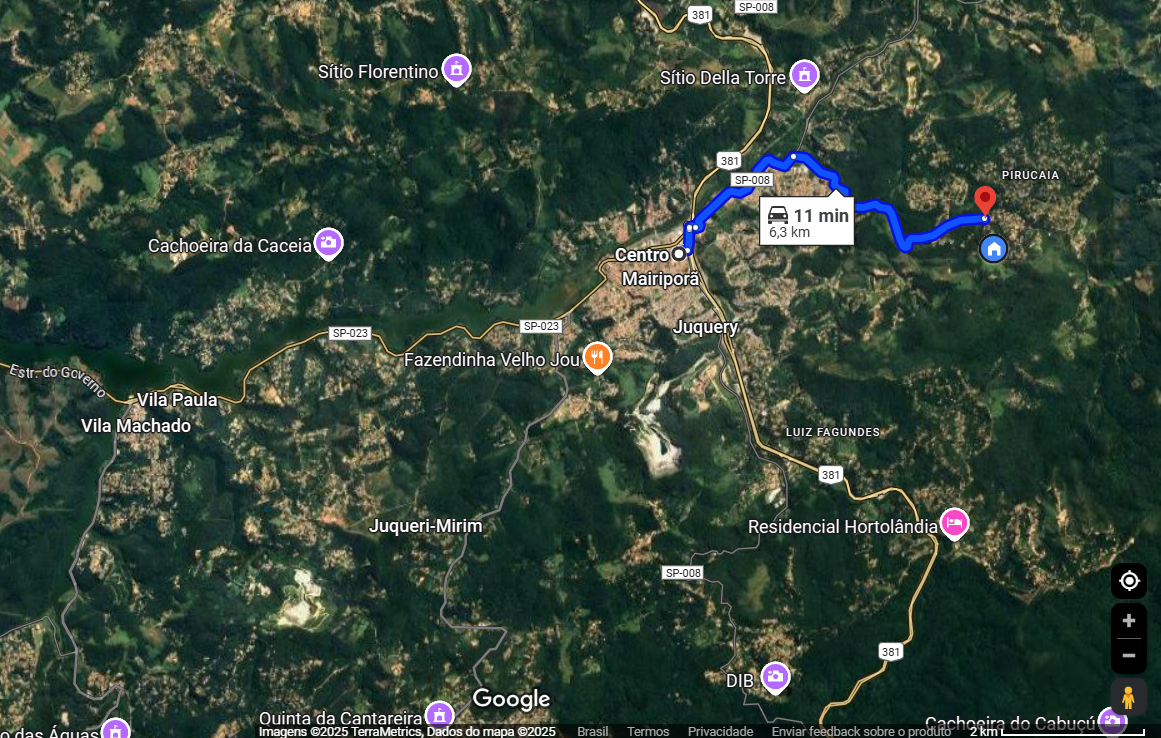
\includegraphics[width=\linewidth]{img/RotaCeuAzulCentro.png}
    \caption{Distância entre o Residencial Céu Azul e o centro de Mairiporã, SP.}
    \legend{Fonte: GoogleMaps.}
    \label{fig:locCeuAzul}
\end{figure}

\begin{figure}[htbp!]
    \centering
    \suppressfloats[t]
    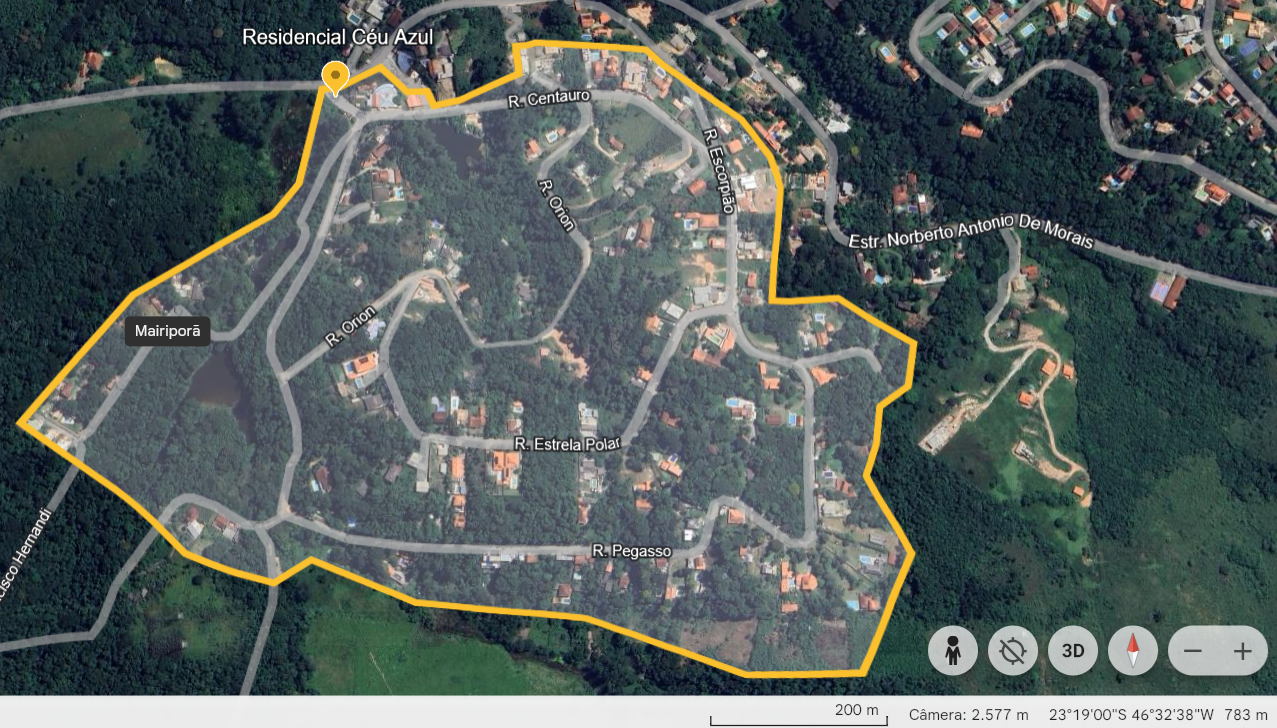
\includegraphics[width=\linewidth]{img/LimitesCeuAzul.png}
    \caption{Limites do Bairro Residencial Céu Azul em Mairiporã, SP.}
    \legend{Fonte: Google Earth com comentário dos autores.}
    \label{fig:limitesCeuAzul}
\end{figure}

Sua administração é composta estaturiamente pelo Conselho Diretor, composto pelo Presidente, Secretário e Tesoureiro, além de um Conselho Fiscal com três assentos, que formalmente fiscaliza a administração e também opina e colabora com as atividades regulares de administração, sendo todas as posições voluntárias e não-remuneradas. Além disto, há a função de Administrador, remunerada, no momento acumulada pelo presidente da associação, não havendo vedação para que o Administrador seja outra pessoa que não o Presidente, ou mesmo não morador. 

Atualmente a Associação possui 107 associados, em sua maioria unidades residenciais unifamiliares, em um loteamento onde a área média dos lotes é de 1.000 m$^2$. Considerando a relação habitante/domicílio de Mairiporã vista na seção \ref{subsec:Contexto}, estima-se uma população permanente de cerca de 300 pessoas em uma área de aproximadamente 43 ha. Além das unidades residenciais individuais, existem também unidades residenciais destinadas a locação de temporada, com pico de ocupação nos feriados e veraneio, chegando a uma população rotativa de 1.000 pessoas nestas épocas do ano.\footnote{As informações referentes ao Residencial Céu Azul nesta seção e nas seguintes foram coletadas em campo pelos autores.}

\section{Delimitação do Problema}\label{sec:Delimitacao}

\subsection{Captação, tratamento e distribuição de água no Recanto Céu Azul}\label{subsec:capAguaCeuAzul}

A captação de água no Residencial Céu Azul se dá por meio de dois poços, sendo um semi-artesiano, com produção de 30 m$^3$/dia e outro artesiano, produzindo 40 m$^3$/dia. Os dois poços funcionam alternadamente, permitindo o repouso das bombas e recarga dos poços sem que haja interrupção da produção. A água captada é enviada a um reservatório de 20 m$^3$ onde recebe tratamento por solução aquosa de hipoclorito de sódio ($\ce{NaClO}$) a 12\%, injetada por meio de uma bomba peristáltica regulada para injeção de 50 ml/h de solução.

A cada ciclo de carga total do reservatório inferior seu conteúdo é recalcado por bombeamento a um reservatório superior com capacidade de 60 m$^3$. Este reservatório está situado no ponto mais alto do bairro, permitindo a distribuição da água por gravidade. O reservatório superior está a uma altitude de 860 m enquanto que o ponto mais baixo do bairro está a cerca de 780 m, permitindo uma pressão de até 80 m.c.a. (784 kPa), em tese muito acima do mínimo exigido pela norma, de 10 m.c.a. \cite{NBR12218}. 

Toda a rede de distribuição é em tubulação de PVC para água fria em diâmetro de 50 mm, diretamente enterrada sob o pavimento de concreto das ruas do bairro, com ramais de conexão às unidades residenciais por tubulação de 25 mm, também em PVC para água fria. Esta rede de distribuição foi construída a cerca de 20 anos pelos moradores, sem assistência técnica especializada e vem sendo mantida pelos mesmos igualmente sem assistência técnica especializada. Estima-se uma grande perda de pressão de distribuição na rede, não só pelo comprimento da tubulação e seu relativamente pequeno diâmetro, mas também pelo uso de conexões do tipo joelho ao invés de curvas de 90$\degree$ ou 45$\degree$ nas mudanças de rumo da tubulação. Vazamentos também são constantes e difícil identificação pelo fato de a tubulação estar enterrada a profundidade relativamente baixa e sofrer com o tráfego de veículos pesados como caminhões de coleta de lixo e entrega de materiais de construção, além de ônibus escolares.

A figura \ref{fig:LinhasDeAgua} mostra a distribuição dos ramais de distribuição de água, conforme relato dos moradores remanescentes da época de sua construção e por inferência a partir das residências atendidas. Cada unidade consumidora é dotada de um hidrômetro, de onde se extrai o consumo para posterior cálculo da tarifa de água cabível a cada unidade consumidora. 

\begin{figure}[htbp!]
    \centering
    \suppressfloats[t]
    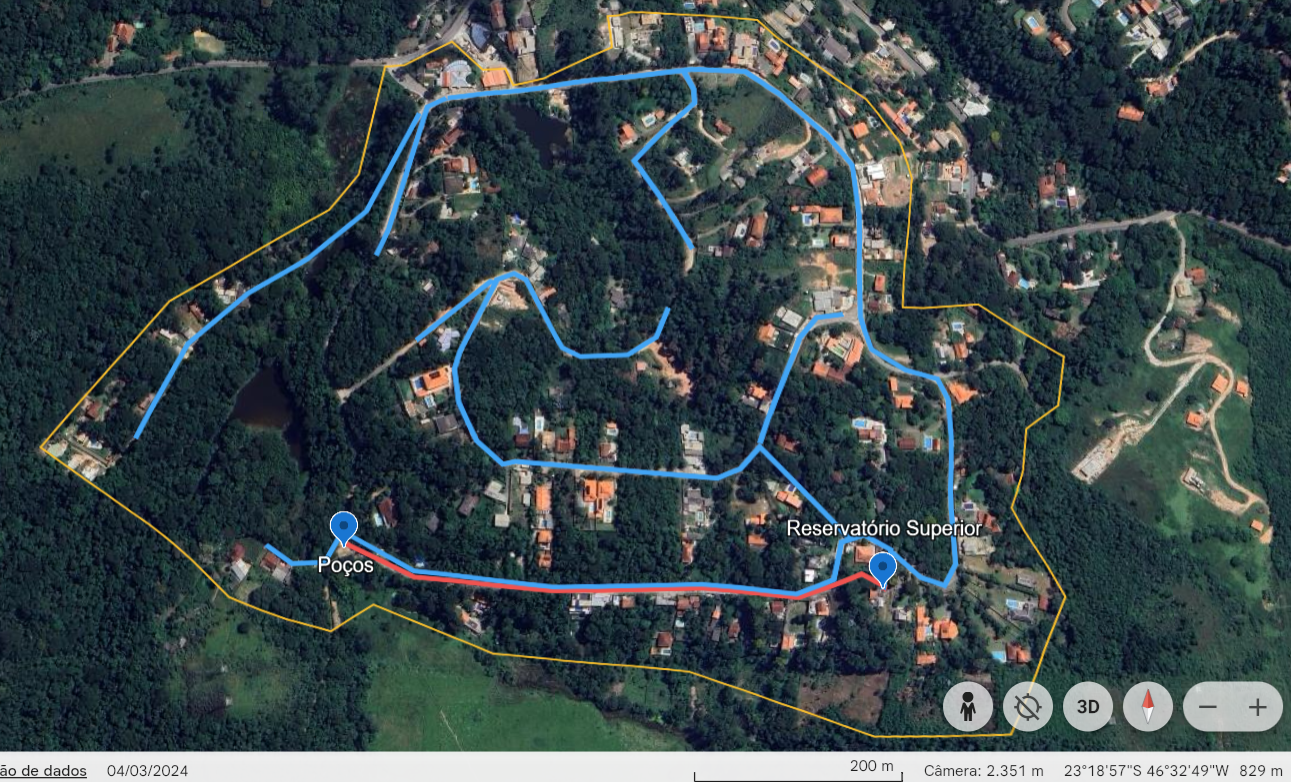
\includegraphics[width=\linewidth]{img/LinhasDeAgua.png}
    \caption{Croqui ilustrativo da localização dos poços de captação de água, reservatório superior, tubulação de recalque de água ao reservatório superior (em vermelho) e ramais de distribuição de água (em azul) do Recanto do Céu Azul.}
    \legend{Fonte: Google Earth com comentário dos autores.}
    \label{fig:LinhasDeAgua}
\end{figure}

A captação de água é insuficiente para o abastecimento e a solulção encontrada pela Associação foi a divisão do circuito em setores, por meio de válvulas esféricas de acionamento manual. Cada setor é abastecido por um nto contínuo da população atendida, e a solução encontrada pela Asperíodo de 3 a 4 horas, a depender do volume de água disponível no reservatório superior, a cada 4 dias. O consumo médio por residência é de 18 m$^3$/mês, de onde se pode estimar que a cota média de água por carga de abastecimento é de 2,4 m$^3$ por residência.

Isto leva a crer que dispor de uma interface que possibilite admnistração e publicação da captação e consumo de água é um problema crítico para o bom convívio e suprimento de uma necessidade básica que é a disponibilidade de água.

\section{Pesquisa de campo}

As hipóteses levantadas nas seções \ref{sec:Justificativa} e \ref{sec:Delimitacao} carecem de validação. Para esta validação foi elaborado formulário de pesquisa na plataforma Google Forms\footnote{https://docs.google.com/forms}, com perguntas elaboradas para avaliar a percepção da comunidade alvo sobre o abastecimento de água. Buscou-se avaliar dois quesitos:
\begin{enumerate}
    \item A restrição de abastecimento de água é um problema real?
    \item Maneiras de melhor administrar o abastecimento de água são interessantes?
\end{enumerate}

As perguntas não foram diretas, mas sim procurou-se avaliar a percepção geral da comunidade, sem perguntar diretamente o que se queria avaliar e evitando-se tendências. As figuras \ref{fig:Form0} a \ref{fig:Form4} mostram as telas do formulário de pesquisa.

\begin{figure}[htbp!]
    \centering
    \suppressfloats[t]
    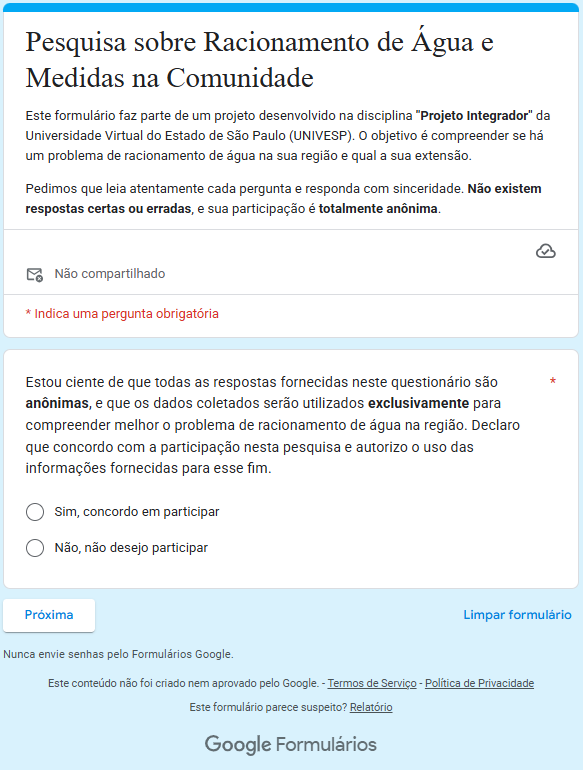
\includegraphics[width=.35\linewidth]{img/FormPesquisa/Form0.png}
    \caption{Página inicial do formulário de pesquisa de capmo sobre a pertinência do projeto.}
    \legend{Fonte: Elaborado pelos autores.}
    \label{fig:Form0}
\end{figure}

\begin{figure}[htbp!]
    \centering
    \suppressfloats[t]
    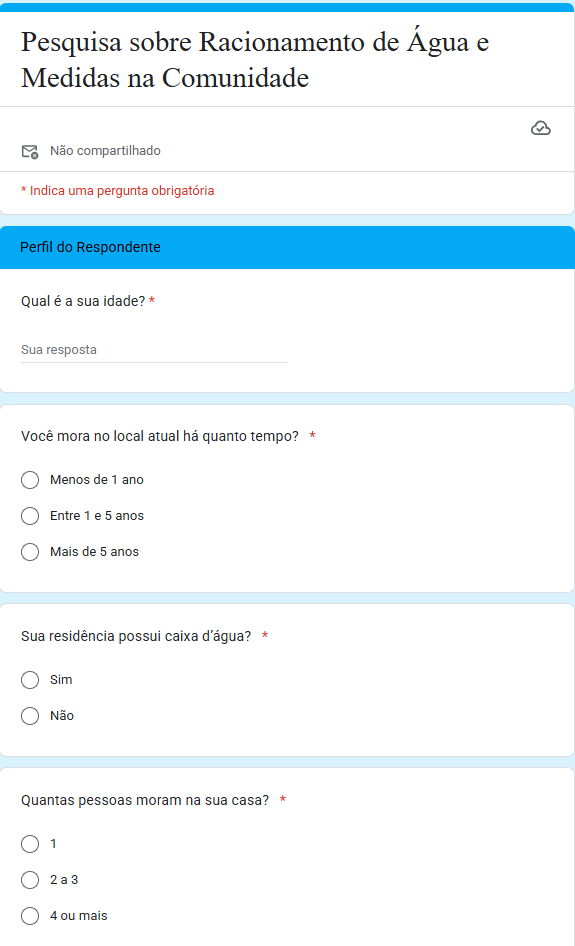
\includegraphics[width=.35\linewidth]{img/FormPesquisa/Form1.png}
    \caption{Segunda página do formulário de pesquisa de capmo sobre a pertinência do projeto.}
    \legend{Fonte: Elaborado pelos autores.}
    \label{fig:Form1}
\end{figure}

\begin{figure}[htbp!]
    \centering
    \suppressfloats[t]
    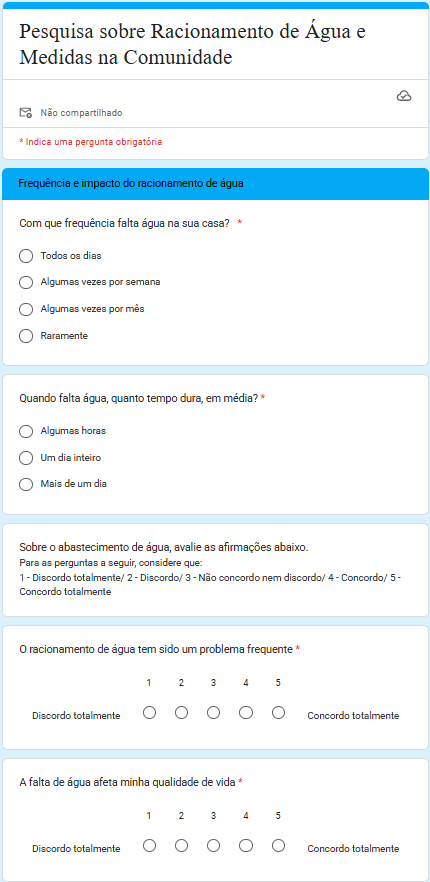
\includegraphics[width=.35\linewidth]{img/FormPesquisa/Form2.png}
    \caption{Terceira página do formulário de pesquisa de capmo sobre a pertinência do projeto.}
    \legend{Fonte: Elaborado pelos autores.}
    \label{fig:Form2}
\end{figure}

\begin{figure}[htbp!]
    \centering
    \suppressfloats[t]
    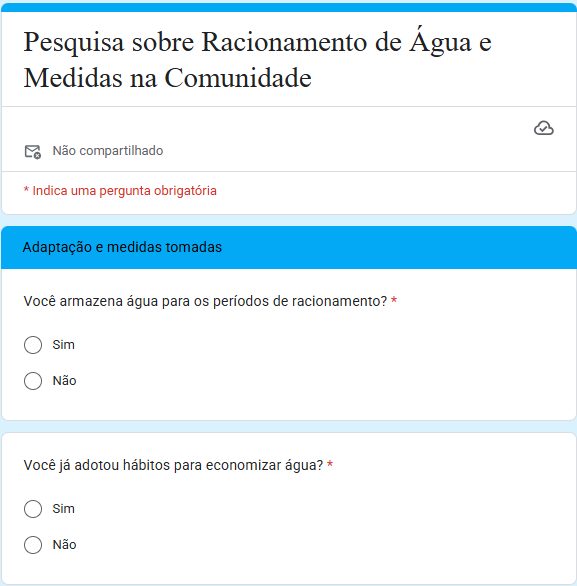
\includegraphics[width=.35\linewidth]{img/FormPesquisa/Form3.png}
    \caption{Quarta página do formulário de pesquisa de capmo sobre a pertinência do projeto.}
    \legend{Fonte: Elaborado pelos autores.}
    \label{fig:Form3}
\end{figure}

\begin{figure}[htbp!]
    \centering
    \suppressfloats[t]
    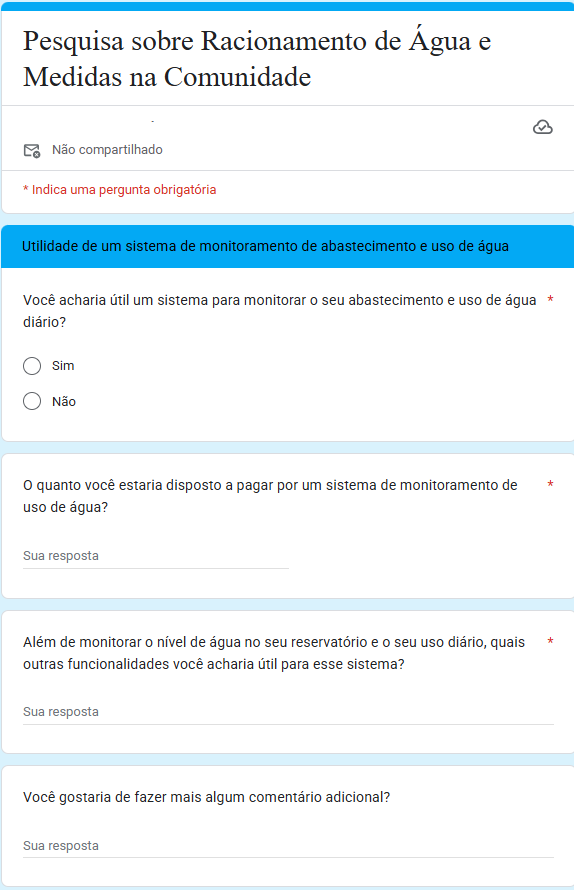
\includegraphics[width=.35\linewidth]{img/FormPesquisa/Form4.png}
    \caption{Página final do formulário de pesquisa de capmo sobre a pertinência do projeto.}
    \legend{Fonte: Elaborado pelos autores.}
    \label{fig:Form4}
\end{figure}

O formulário foi disponibilizado a todos os associados, através do grupo de WhatsApp da comunidade e, dos 105 associados, obtiveram-se 76 respondentes.



\section{Metodologia}\label{sec:Metodologia}

\subsection{Caso de uso}\label{subsec:casoDeUso}

O primeiro passo para o desenvolvimento da solução foi definir as funcionalidades do sistema e os respectivos usuários que as executariam. Para isso, foi elaborado um Diagrama de Caso de Uso (figura \ref{fig:DiagCasoUso}) seguindo os padrões da linguagem \textbf{UML} (\textit{Unified Modeling Language}). \cite{umlGuia}

\begin{figure}[htbp!]
    \centering
    \suppressfloats[t]
    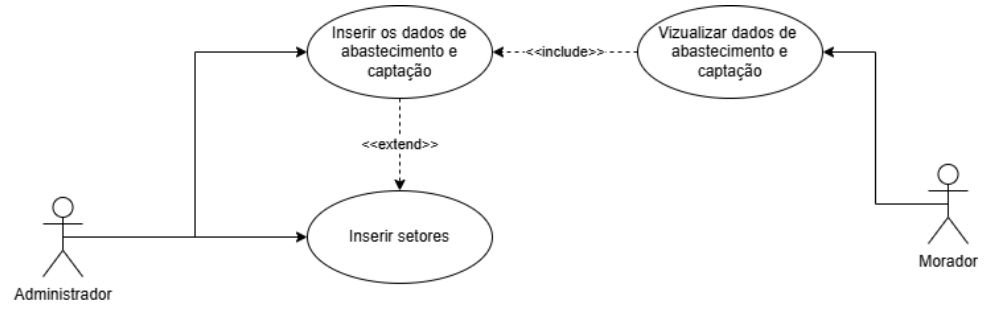
\includegraphics[width=\linewidth]{img/DiagCasoUso.png}
    \caption{Diagrama de Caso de Uso para a aplicação em desenvolvimento.}
    \legend{Fonte: Elaborado pelos autores.}
    \label{fig:DiagCasoUso}
\end{figure}

Definiu-se que o sistema possuiria três casos de uso. O primeiro consiste na \textbf{inserção de dados de abastecimento e captação}, ação realizada por um ator do tipo \textbf{Administrador}. Esse caso de uso pode estar condicionado ao caso em que o administrador insere os \textbf{setores abastecidos pelo sistema}. Essa relação de dependência é representada pela associação \verb|<<extend>>|. \cite{larman}

O terceiro caso de uso contempla a \textbf{visualização dos dados de abastecimento e captação pelos moradores}, e está condicionado à existência de dados inseridos previamente pelo administrador. Essa dependência é representada pelo relacionamento \verb|<<include>>|. \cite{fowler}

\subsection{Modelagem de Dados}\label{subsec:Modelagem}

Com os casos de uso bem definidos, partiu-se para a modelagem de dados. Foi elaborado o \textbf{Modelo de Entidades e Relacionamentos (MER)}, conforme recomendações de \citeonline{heuser} apresentado na figura \ref{fig:MER}.



\begin{figure}[htbp!]
    \centering
    \suppressfloats[t]
    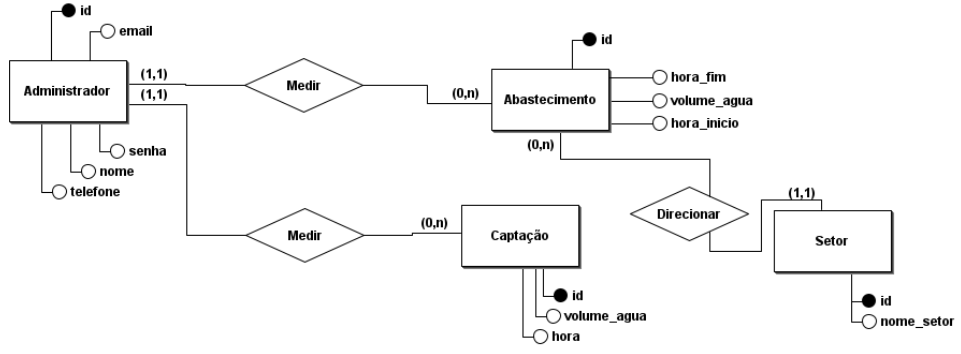
\includegraphics[width=\linewidth]{img/MER.png}
    \caption{Modelo de Entidades e Relacionamentos para a aplicação em desenvolvimento.}
    \legend{Fonte: Elaborado pelos autores.}
    \label{fig:MER}
\end{figure}

Foram definidas quatro entidades: \textbf{Administrador}, \textbf{Abastecimento}, \textbf{Captação} e \textbf{Setor}. Todas as entidades possuem um \textbf{identificador (ID)} único do tipo inteiro. A entidade \textit{Administrador} possui, adicionalmente, os atributos: nome, \textit{e-mail}, \textit{telefone} e \textit{senha}.

A entidade \textit{Abastecimento} armazena os dados referentes à \textbf{hora de início e fim do abastecimento} e o \textbf{volume de água abastecida}. Já a entidade \textit{Captação} registra o \textbf{volume captado} e a \textbf{hora de aferição}.

As entidades \textit{Abastecimento} e \textit{Captação} estão relacionadas à entidade \textit{Administrador} para identificar qual usuário inseriu os dados. Trata-se de um relacionamento 1:1 do lado do \textit{Administrador}, pois cada registro de abastecimento ou captação é feito por um único administrador. Contudo, um administrador pode realizar nenhum ou vários registros, caracterizando um relacionamento de 0:N do lado de \textit{Abastecimento} e \textit{Captação}. \cite{heuser}

Por fim, cada registro de \textit{Abastecimento} está vinculado a \textbf{um único Setor}, enquanto um \textit{Setor} pode ter recebido vários abastecimentos, ou mesmo nenhum.

\subsection{Modelo Lógico e Físico}\label{subsec:nodeloLogicoFisico}

Com o MER concluído, foi elaborado o \textbf{Diagrama de Entidades e Relacionamentos (DER)} \cite{dateBD} representando o modelo lógico do banco de dados (figura \ref{fig:DER}).

\begin{figure}[htbp!]
    \centering
    \suppressfloats[t]
    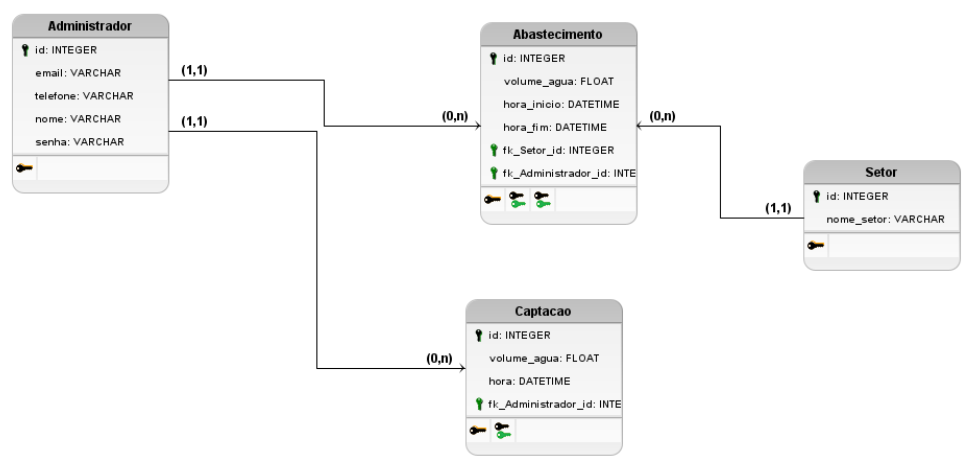
\includegraphics[width=\linewidth]{img/DER.png}
    \caption{Diagrama de Entidades e Relacionamentos para a aplicação em desenvolvimento.}
    \legend{Fonte: Elaborado pelos autores.}
    \label{fig:DER}
\end{figure}

Nos três relacionamentos definidos no MER, a cardinalidade foi estabelecida como \textbf{$(1, 1) - (0, n)$}. De acordo com a teoria de banco de dados relacionais \cite{heuser}, a \textbf{chave estrangeira} deve ser inserida na tabela correspondente ao lado da cardinalidade $(0, n)$, referenciando o identificador da entidade do lado $(1, 1)$.

Assim, temos:
\begin{itemize}
    \item A tabela \textit{Abastecimento} contém uma chave estrangeira que referencia a tabela \textit{Administrador};
    \item A tabela \textit{Captação} também contém uma chave estrangeira para \textit{Administrador};
    \item A tabela \textit{Abastecimento} possui ainda uma chave estrangeira para \textit{Setor}.
\end{itemize}

Definiram-se também os tipos de dados:
\begin{itemize}
    \item Todos os \textbf{IDs} foram definidos como \verb|INTEGER|;
    \item Na tabela \textit{Administrador}, os atributos \textit{nome}, \textit{e-mail}, \textit{telefone} e \textit{senha} foram definidos como \verb|VARCHAR|, tipo adequado para armazenar textos com tamanho variável \cite{heuser};
    \item Os atributos \textit{volume de água} (captação e abastecimento) foram definidos como \verb|FLOAT|, conforme prática comum para valores numéricos com ponto flutuante \cite{dateBD};
    \item Os atributos \textit{hora de início}, \textit{hora de fim} e \textit{hora de aferição} foram definidos como \verb|DATETIME|, tipo de dado apropriado para armazenar informações de data e hora com precisão \cite{dateBD};
    \item O nome do \textit{Setor} também foi definido como \verb|VARCHAR| por ser um campo textual \cite{heuser}.
\end{itemize}

Concluída a modelagem de dados, iniciou-se a implementação do banco de dados utilizando o \textbf{\textit{MySQL}}, um sistema de gerenciamento de banco de dados relacional amplamente utilizado e de código aberto.



\subsection{Desenvolvimento da aplicação}\label{subsec:DesAplic}

A partir da familiaridade dos autores com a linguagem \textit{Java}, foi escolhido o \textit{framework} \textit{\textbf{Spring Boot}}\footnote{https://spring.io/projects/spring-boot} para o desenvolvimento do \textit{backend} da aplicação. \cite{walls}

Antes da implementação das interfaces, foram criados os \textit{wireframes} (representações estruturais e simplificadas das telas do sistema) que definem a organização dos elementos de interface, a hierarquia de informações e os fluxos de navegação \cite{garret} (figuras \ref{fig:wireframe1}, \ref{fig:wireframe2} e \ref{fig:wireframe3}). A utilização de wireframes permitiu uma prototipagem rápida e alinhada às funcionalidades previamente definidas.

\begin{figure}[htbp!]
    \centering
    \suppressfloats[t]
    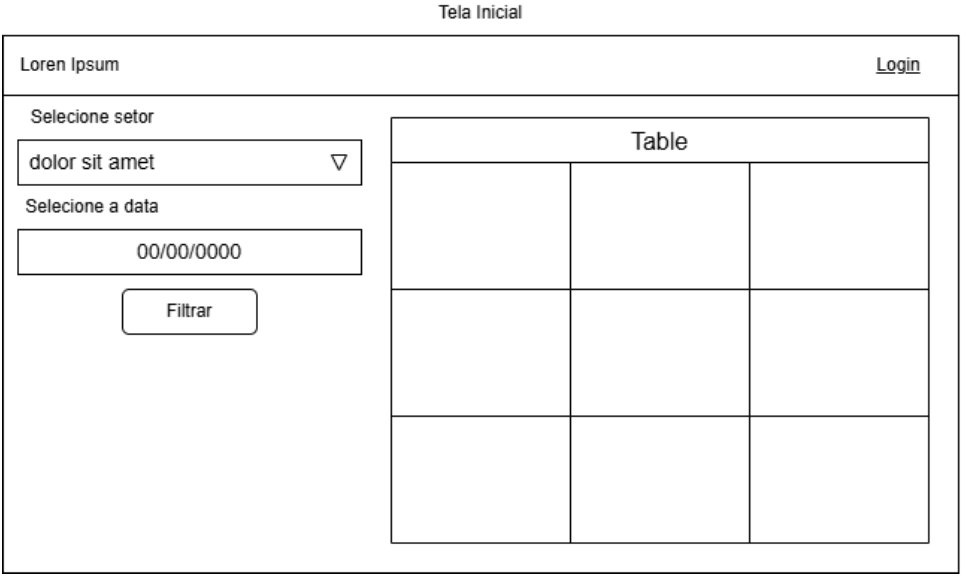
\includegraphics[width=\linewidth]{img/wireframe1.png}
    \caption{Wireframe da tela inicial da aplicação.}
    \legend{Fonte: Elaborado pelos autores.}
    \label{fig:wireframe1}
\end{figure}

\begin{figure}[htbp!]
    \centering
    \suppressfloats[t]
    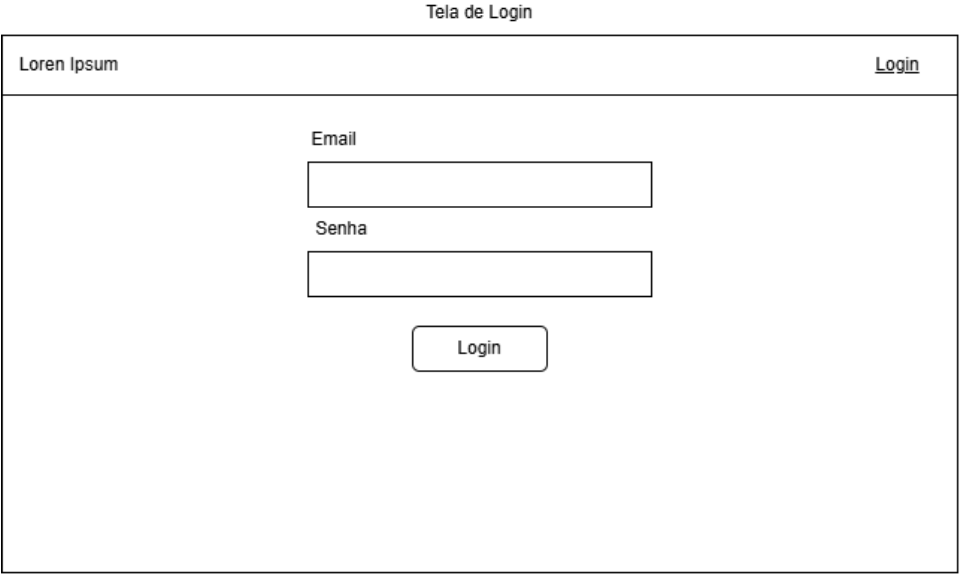
\includegraphics[width=\linewidth]{img/wireframe2.png}
    \caption{Wireframe da tela de login da aplicação.}
    \legend{Fonte: Elaborado pelos autores.}
    \label{fig:wireframe2}
\end{figure}

\begin{figure}[htbp!]
    \centering
    \suppressfloats[t]
    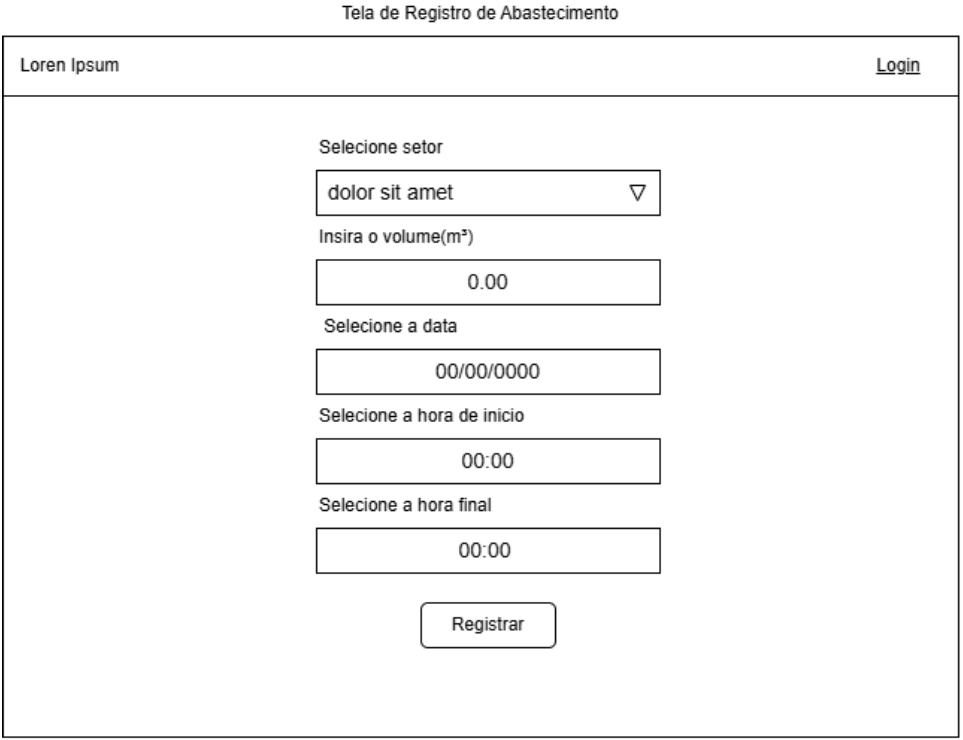
\includegraphics[width=\linewidth]{img/wireframe3.png}
    \caption{Wireframe da tela de registro de abastecimento da aplicação.}
    \legend{Fonte: Elaborado pelos autores.}
    \label{fig:wireframe3}
\end{figure}

Com os wireframes prontos, as interfaces foram convertidas em páginas HTML estáticas, utilizando \textbf{HTML5}, \textbf{CSS3} e \textbf{JavaScript}, com o auxílio do framework de componentes visuais Bootstrap 5, que oferece recursos prontos para responsividade, estilização e organização visual das páginas \cite{bootstrap}. As figuras \ref{fig:tela1}, \ref{fig:tela2} e \ref{fig:tela3} trazem os protótipos das telas de início, login e entrada de dados, respectivamente.
 
\begin{figure}[htbp!]
    \centering
    \suppressfloats[t]
    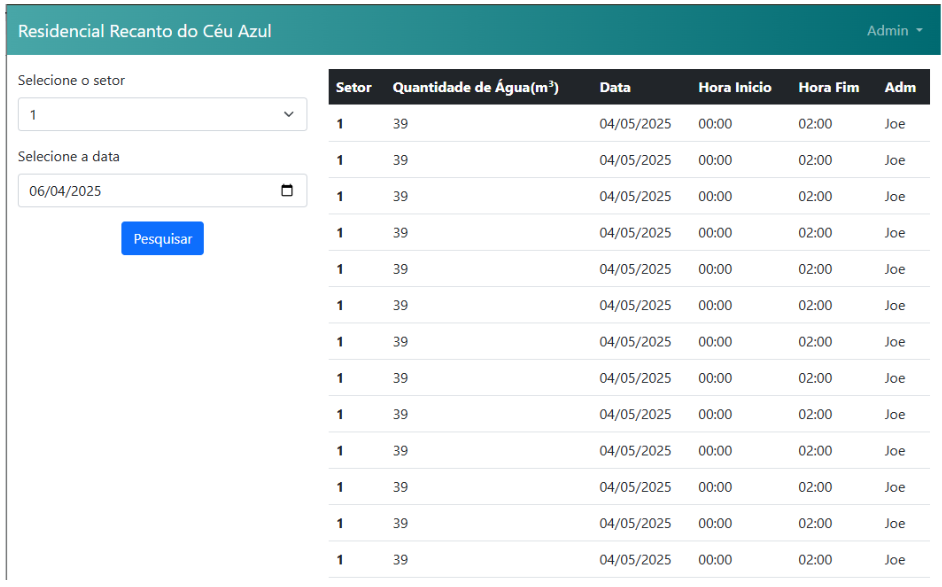
\includegraphics[width=\linewidth]{img/tela1.png}
    \caption{Protótipo da tela inicial da aplicação.}
    \legend{Fonte: Elaborado pelos autores.}
    \label{fig:tela1}
\end{figure}

\begin{figure}[htbp!]
    \centering
    \suppressfloats[t]
    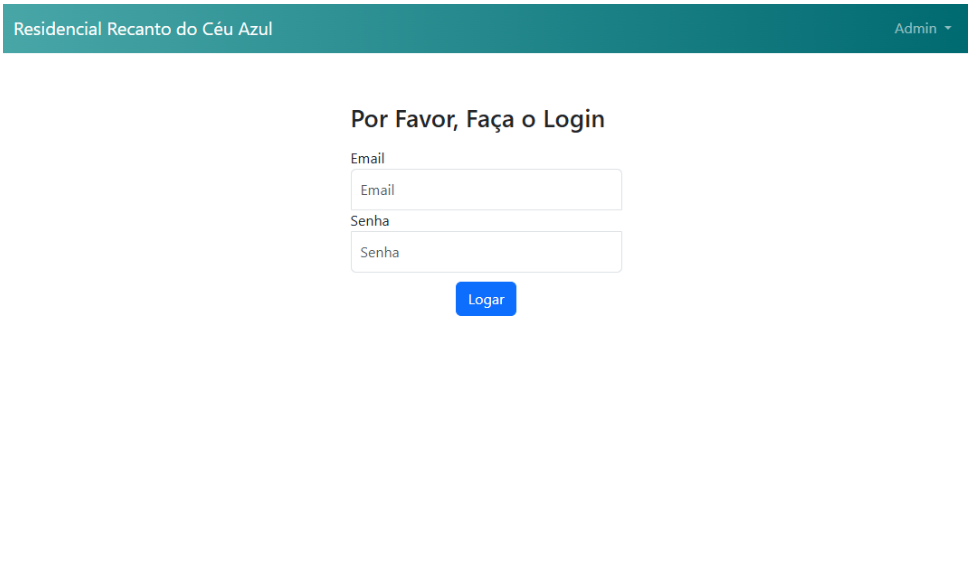
\includegraphics[width=\linewidth]{img/tela2.png}
    \caption{Protótipo da tela de login da aplicação.}
    \legend{Fonte: Elaborado pelos autores.}
    \label{fig:tela2}
\end{figure}

\begin{figure}[htbp!]
    \centering
    \suppressfloats[t]
    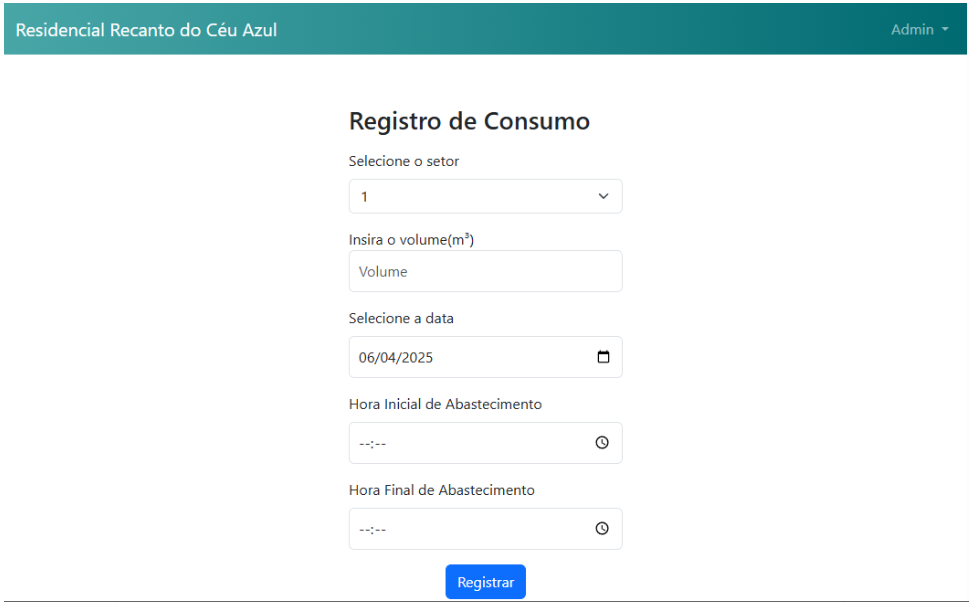
\includegraphics[width=\linewidth]{img/tela3.png}
    \caption{Protótipo da tela de registro de abastecimento da aplicação.}
    \legend{Fonte: Elaborado pelos autores.}
    \label{fig:tela3}
\end{figure}


O projeto adotou a arquitetura \textbf{Model-View-Controller (MVC)}, um padrão de desenvolvimento que separa a lógica de negócio (\textit{Model}), a interface com o usuário (\textit{View}) e o controle das requisições (\textit{Controller}). \cite{sommerville}

\section{Próximos passos}\label{sec:proxPassos}

Com o banco de dados e as views definidos, os próximos passos incluem a elaboração das classes de modelo (\textit{Model}), responsáveis pela conexão com o banco de dados e manipulação das informações, e das classes de controle (\textit{Controller}), que irão gerenciar as requisições dos usuários e invocar os respectivos \textit{Models} e \textit{Views}.
    

    % Elementos pós-textuais
    \postextual

    \bibliography{RelatorioParcial}

\end{document}
